\documentclass[conference, 11pt]{IEEEtran}
\usepackage{xcolor}
\usepackage{cite}
\usepackage{url}
\usepackage{graphicx}
\usepackage{enumitem}
\usepackage{parskip}
\usepackage{booktabs}
\usepackage{graphicx}
\usepackage{pdfpages}
\usepackage[font=small,labelfont=bf]{caption}
\usepackage[font=small,labelfont=bf]{subcaption}

\begin{document}
\newcommand{\derek}[1] {\textcolor{blue}{\textbf{[Derek: #1]}}}
\newcommand{\mina}[1] {\textcolor{green}{\textbf{[Mina: #1]}}}
\newcommand{\mazyar}[1] {\textcolor{orange}{\textbf{[Mazyar: #1]}}}
\newlist{questions}{enumerate}{2}
\setlist[questions,1]{label=RQ\arabic*.,ref=RQ\arabic*}
\setlist[questions,2]{label=(\alph*),ref=\thequestionsi(\alph*)}

\title{Phylogenetic and Structural Analysis of BC200 and \emph{Hominoidea} Homologs}

\author{Derek Robinson, Mina Emadi, Mazyar Ghezelji\\
University of Victoria\\
Victoria, Canada \\
\{drobinson, minaemadi, mazyarghezelji\}@uvic.ca}

\maketitle

\begin{abstract}
Alzheimer’s disease (AD) is a neurodegenerative disorder resulting from synaptic plasticity failure in neurons, which greatly affects the cognitive ability of patients. 
AD is linked to the accumulation of beta-amyloid protein and tau protein, which in abnormal levels can disrupt cell functions and potentially lead to diseases such as AD. 
Previous studies have suggested that AD is a uniquely human disease. 
In this paper, we investigate this claim by analyzing genetic similarities between humans and other species of the \emph{Hominoidea} superfamily.
We break down our problem into two crucial parts; performing phylogenetic analysis of a long non-coding RNA associated with AD named Brain Cytoplasmic 200 lncRNA (BC200), and investigating the structural differences between BC200 and its four most closely related \emph{Hominoidea} homologs. 
We start by first performing a NCBI Blast search to determine similar sequences, followed by building a phylogenetic tree to determine closely related homologs.
We then observe the most similar sequences and build their secondary structures, which are then used to compare functions of BC200 and its homologs.
Although these sequences are similar, secondary structure comparison revealed structural differences between human BC200 and its homologs, meaning that they may exert different functions in the body.
As a result, our findings neither support nor refute that AD is a uniquely human disease.
\end{abstract}

\section{Introduction}\label{sec:intro}

Alzheimer's disease (AD) is a neurodegenerative disease which greatly affects the lives of those who are diagnosed and those who care for the diagnosed. 
In the United States, 6.2 million patients are estimated to be living with AD and it is the sixth leading cause of death for American adults \cite{AlzheimersDisease}. 
In Canada, over 747,000 patients are living with AD, or another form of dementia \cite{ADcanada}. 
In mild cases, patients with AD may exhibit memory loss and poor judgement \cite{alzheimersSigns}. 
The symptoms of higher severity cases may include the the inability to communicate, seizures, and difficulty swallowing \cite{alzheimersSigns}.

AD involves multiple cell types and signaling pathways \cite{zhang2021role}. 
As such, the collective knowledge of AD is spread across many different domains. 
This spread of knowledge means that fully understanding AD in humans is difficult, let alone attempting to understand if the disease affects other species of the \emph{Hominoidea} superfamily.
Finch and Austad argue that with our current understanding of AD, it is not possible to determine if AD is uniquely human \cite{finch2015commentary}. 
Thus, this paper explores one facet of AD pathogenesis, the long non-coding RNA (lncRNA) BC200. 
BC200 has been implicated in AD bu upregulating the expression of b-site APP-cleaving enzyme1 (BACE1) \cite{li2018identification,zhang2021role}. 
The upregulation of BACE1 in turn leads to higher levels of beta-amyloid (A$\beta$) in the brain, which can forms plaques, accumulate in neurons, and disrupt cell function. \cite{li2018identification,zhang2021role}. 

In hopes of better understanding the role that \emph{Hominoidea} homologs of BC200 play in AD, we answer the following research questions:

\begin{questions}
  \item What does the phylogenetic tree of BC200 look like?
  \item What structural differences exist between BC200 and its four most closely related \emph{Hominoidea} homologs?
\end{questions}

The remainder of this paper is structured as follows: section \ref{sec:background} gives background into BC200 and the role it plays in AD, section \ref{sec:methods} lays out the methods used for selecting BC200 homologs and performing both the phylogenetic structural analysis, section \ref{sec:results} presents the results of our analysis, section \ref{sec:discussion} discusses the relevancy of the results, and section \ref{sec:conclusion} concludes the paper.

\section{Background}\label{sec:background}

\subsection{What is BC200?}

BC200, sometimes referred to as BCYRN1, is a 200 nucleotide long RNA transcript which is found predominantly in the brain \cite{tiedge1993primary}. 
As a lncRNA, BC200 is not translated into protein, but can be used as a potential therapeutic target and biomarker due to its regulatory role in biological processes involved in disease development \cite{zhang2021role,mus2007dendritic}. 
This lncRNA has recently been studied extensively due to its regulatory role in translation, as well as its pathogenic impact in AD \cite{zhang2021role,tiedge1993primary}. 
Because of the crucial role BC200 plays in translation control, it impacts the synthesis of dendritic proteins which facilitates long-term plastic changes at the synapse \cite{mus2007dendritic}.

\subsection{The Relation Between AD and BC200}

AD is a neurodegenerative disease resulting from synaptic plasticity failure in neurons \cite{mus2007dendritic}. 
One protein implicated in the onset of AD is beta-amyloid. 
A$\beta$, a cleavage product of the amyloid precursor protein (APP), is generated by b-site APP-cleaving enzyme1 (BACE1) and $\gamma$-secretase complex. 
Beta-amyloid strongly influences the pathogenesis of AD due to the formation of plaques, accumulation in neurons, and disruption of cell functions. 
BC200 facilitates AD pathogenesis by increasing A$\beta$ production through the upregulation of BACE1 expression. 
The inhibition of BC200 significantly suppresses BACE1 expression, increases cell viability and reduces cell apoptosis in an AD model, and these effects are reversed by BC200 over-expression \cite{li2018identification,zhang2021role}. Inhibition of BACE1 activity subsequently leads to a reduction in A$\beta$ levels and may cure or prevent AD \cite{li2018identification,zhang2021role}.

Many researches have demonstrated the important role of BC200 in AD. 
Mus \emph{et al.} show that there is a steady decline in BC200 levels from ages 49 to 86, but a substantially higher amount was detected in AD patients \cite{mus2007dendritic}. 
They also observe that BC200 expression is increased in brain areas that are implicated in AD and it is correlated with disease severity. 
Li \emph{et al.} establish an AD cell model which over-expresses A$\beta$ 1-42 to observe the effects of BC200 on cell viability on cell viability, apoptosis, and to investigate it's mechanistic role on these processes \cite{li2018identification}. 
They observe that knockdown of BC200 led to an increase in cell viability and a decrease in cell apoptosis via the mediation of BACE1.
Inhibition of BC200 rescued this A$\beta$ 1-42 mediated dysfunction, as indicated by the interaction of BC200 directly targeting BACE1. 
Moreover, inhibition of BC200 increased AD cell growth and reduced cell apoptosis. 
They demonstrate that BC200 is a potent positive regulator of BACE1 in AD cells and in conclusion, lncRNA BC200 facilitates AD pathogenesis by up-regulating A$\beta$ through BACE1.

\subsection{What are Alu domains and what is their role in body?}

Alu domains (or elements) are sections of RNA which are responsible for for the regulation of tissue-specific genes. 
Additionally, they are involved in the transcription of nearby genes and may change the expression of said gene. 
In some cases,  Alu domains can be detrimental and result in inherited disorders such as AD, Lung cancer, and Gastric cancer \cite{tseng2013oxidative}. 

\subsection{Sequence Conservation}

Over many generations, random mutations and deletions can change nucleic acid sequences in the genome of an evolutionary lineage. 
Chromosomal rearrangement may also recombine or delete sequences. 
Conserved sequences are sequences which persist in the genome despite such forces, and have slower rates of mutation than the background mutation rate\cite{kimura1974some}. 
Non-coding sequences important for gene regulation, such as the binding or recognition sites of ribosomes and transcription factors, may be conserved within a genome. For example, the promoter of a conserved gene or operon may also be conserved.

\section{Materials and Methods}\label{sec:methods}

The methodology workflow we followed is presented in Fig. \ref{fig:methods}.

\begin{figure*}[ht]
  \centering
  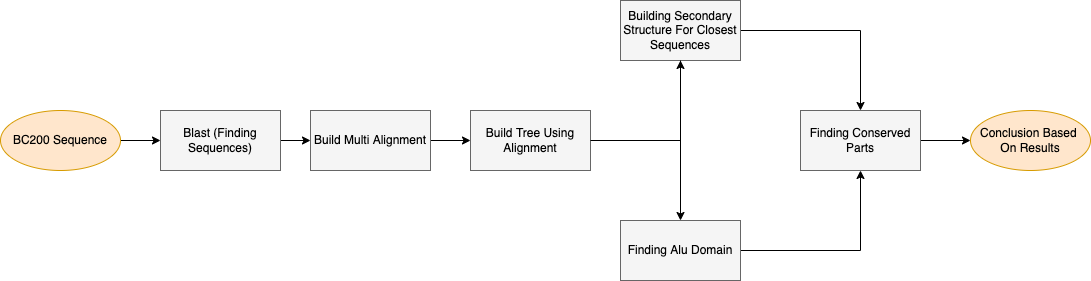
\includegraphics[width=\textwidth, keepaspectratio]{figs/workflow.png}
  \caption{Methodology Workflow}
  \label{fig:methods}
\end{figure*}

\subsection{Selection of lncRNAs}\label{sec:lncRNA-selection}

The lncRNA BC200 was selected for phylogenetic and structural analysis due to the role it plays in AD as discussed in section \ref{sec:background}. 
The homologs of BC200 were selected as a result of an NCBI Blast \cite{blastTool} search. 
Specifically, Megablast \cite{morgulis2008database} with default parameters was used as it is able to compare closely related sequences \cite{amirmahani2018phylogenetic}. 
From the Blast results, the top six sequences of known BC200 homologs were chosen , identified by the inclusion of BC200 in their name. 
Two of the top hits in the Blast results were complete bacterial artificial chromosome sequences for \emph{Pan troglodytes}. 
Inclusion of these two sequences (accession numbers: AC185986.3, AC183594.3) caused errors in the analysis software described in section \ref{sec:phylo} and section \ref{sec:structure}, as such we did not consider these full chromosome sequences in our analysis. 
Table \ref{tbl:accession} outlines the organism names and accession numbers for each of the chosen sequences. 

\begin{table}[ht]
  \centering
  \caption{lncRNA Sequence Information}
  \label{tbl:accession}
  \begin{tabular}{lc}
    \toprule
    Organism Name & Sequence Accession Number \\
    \midrule
    \emph{Homo sapiens}    & NR\_001568.1 \\
    \emph{Pongo pygmaeus}  & AF067780.1 \\
    \emph{Pan paniscus}    & AF067778.1 \\
    \emph{Gorilla gorilla} & AF067779.1 \\
    \emph{Macaca mulatta}  & AF067784.1 \\
    \emph{Hylobates lar}   & AF067781.1 \\
    \emph{Papio hamadryas} & AF067782.1 \\
    \bottomrule
  \end{tabular}
\end{table}

\subsection{Phylogenetic Analysis}\label{sec:phylo}

The lncRNA sequences in Table \ref{tbl:accession} were subject to phylogenetic analysis.
The phylogenetic tree was built using the MEGA11 \cite{tamura2021mega11} bioinformatics software. 
The sequences outlined in Table \ref{tbl:accession} were aligned using the MEGA11 alignment module. 
The multiple sequence alignment was performed using the MUSCLE algorithm \cite{edgar2004muscle} with default parameters in the MEGA11 alignment module. 
Once the multiple sequence alignment had been performed, it was then possible to build the phylogenetic tree. 

The phylogenetic tree was built using the maximum likelihood statistical method and Tamura-Nei substitution model \cite{tamura1993estimation, tamura2004prospects}. 
The bootstrap method was used as a test of phylogeny with 500 replications.
In order to further support the phylogenetic tree, estimates of evolutionary divergence were also calculated by MEGA11 \cite{tamura2021mega11}. 
Evolutionary divergence estimates were calculated using Maximum Composite Likelihood and the Tamura-Nei model \cite{tamura1993estimation, tamura2004prospects}. 
All ambiguous positions were removed for each sequence pair (pairwise deletion option). 

\subsection{Structural Analysis}\label{sec:structure}

In order to approximate the RNA secondary structure of BC200 and four of its closest homologs, we used FORNA, a platform which estimates RNA secondary structure \cite{kerpedjiev2015forna}. 
FORNA is able to draw the RNA secondary structure from the dot bracket notation provided by the user or approximate the minimum free energy (MFE) structure as calculated by RNAFold \cite{lorenz2011viennarna}. 
As this analysis aims at computationally determining a secondary structure, the latter option of using the MFE structure was employed. 
Using structural similarity as a metric for functional similarity, we compared the structure of BC200 to its homologs.
The approximated BC200 structure consists of three main domains, the Alu, A-rich, and unique domain. 
Comparing each homolog structure into BC200, we divided them to three main domains as seen in the BC200 structure and analyzed structural differences in each domain.

\subsection{Finding Alu Domains}

In order to find the Alu domains present in our sequences, we used Dfam \cite{storer2021dfam}. 
The Dfam database is an open collection of Transposable Element DNA sequence alignments, hidden Markov Models (HMMs), consensus sequences, and genome annotations. 
By using the sequence search we identified the Alu domains of the BC200 and its homologs. 
We performed a sequence search for each of the target lncRNAs and compared the first row names of the diagram for each sequence search. 
Comparing the Alu domain structure gives us a suitable result for the RNA function.

\subsection{Finding Conserved Parts of BC200}

One of the best ways for visualize conserved sequences during evolution, is multiple sequence alignment. 
Here, we aligned BC200 and the four most related homologs with each other to find the conserved parts of the sequence. 
We used Clustal Omega for aligning the sequences \cite{madeira2019embl}. 
The CLUSTAL format includes a plain-text key to annotate conserved columns of the alignment, denoting conserved sequence (*), conservative mutations (:), semi-conservative mutations (.), and non-conservative mutations ( ). 
The guide tree for the multiple sequence alignment is shown in Fig. \ref{fig:Guide-tree}. 
The conservation percentage of BC200 was calculated by comparing the number of conserved nucleotides to number of total nucleotides in the sequence.

\begin{figure}[ht]
  \centering
  
\includegraphics[width=0.55\textwidth]{figs/guidetree.png}
  \caption{Multiple Sequence Alignment Guide Tree}
  \label{fig:Guide-tree}
\end{figure}

\section{Results}\label{sec:results}

\subsection{Phylogenetic Tree of BC200}

The results of the phylogenetic analysis can be found in Fig. \ref{fig:phylo-tree}. 
The tree shows that the \emph{Homo sapiens} BC200 lncRNA and the \emph{Gorilla gorilla} BC200 lncRNA are likely to share a common ancestor. 
Similarly, the BC200 homologs from \emph{Pan paniscus} and \emph{Hylobates lar} are likely to share a common ancestor. 
This is also the case for the BC200 homologs from \emph{Macaca mulatta}, \emph{Papio hamadryas}, and \emph{Pongo pygmaeus}. 

\begin{figure}[ht]
  \centering
  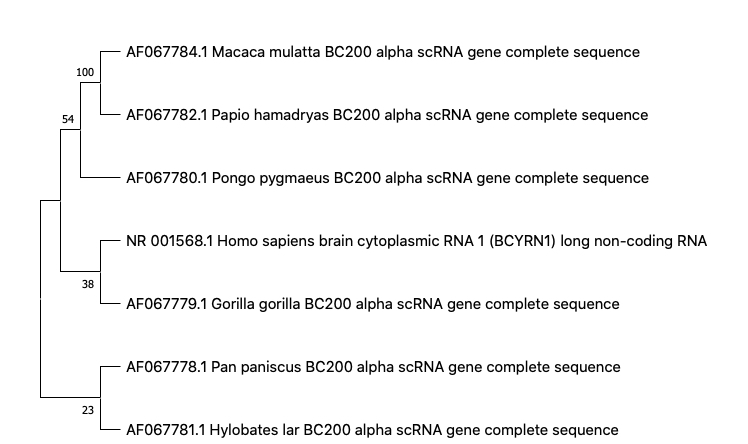
\includegraphics[width=\columnwidth, keepaspectratio]{figs/phylogenetic-tree.jpg}
  \caption{Phylogenetic tree of BC200 and \emph{Hominoidea} homologs. The numbers at each node are the bootstrap support values obtained by maximum likelihood.}
  \label{fig:phylo-tree}
\end{figure}

Additionally, Table \ref{tbl:distances} shows the pairwise distances between sequences which estimate the evolutionary divergence between sequences. 
The evolutionary divergence estimates show that the four most closely related homologs of BC200 found in other \emph{Hominoidea} come from \emph{Pan paniscus} (AF067778.1), \emph{Pongo pygmaeus} (AF067780.1), \emph{Hylobates lar} (AF067781.1), and \emph{Gorilla gorilla} (AF067779.1), in order of evolutionary distances. 
Thus, the aforementioned BC200 homologs (AF067778.1, AF067780.1, AF067781.1, AF067779.1) are the closest relatives of BC200 and have their secondary structure analyzed in section \ref{sec:results-structure}.

\begin{table*}[h]
  \centering
  \caption{Estimates of Evolutionary Divergence between Sequences}
  \label{tbl:distances}
  \begin{tabular}{lcccccc}
    \toprule
    Accession Number \\
    \midrule
    NR\_001568.1 \\
    AF067780.1 & 0.01023 \\
    AF067778.1 & 0.00503 & 0.02169 \\
    AF067779.1 & 0.03070 & 0.02890 & 0.01709 \\ 
    AF067784.1 & 0.03088 & 0.04573 & 0.03802 & 0.05235 \\
    AF067781.1 & 0.02561 & 0.02763 & 0.01562 & 0.02439 & 0.04353 \\ 
    AF067782.1 & 0.03120 & 0.04478 & 0.03947 & 0.04731 & 0.00852 & 0.04259 \\
    \bottomrule
  \end{tabular}
\end{table*}

\subsection{Structural difference between BC200 and its homologs}\label{sec:results-structure}

The BC200 structure consist of three main parts: the Alu, A-rich, and unique domain \cite{jung2014rna} as shown in Fig. \ref{fig:bc200-structure}.

\begin{figure}[h]
  \centering
  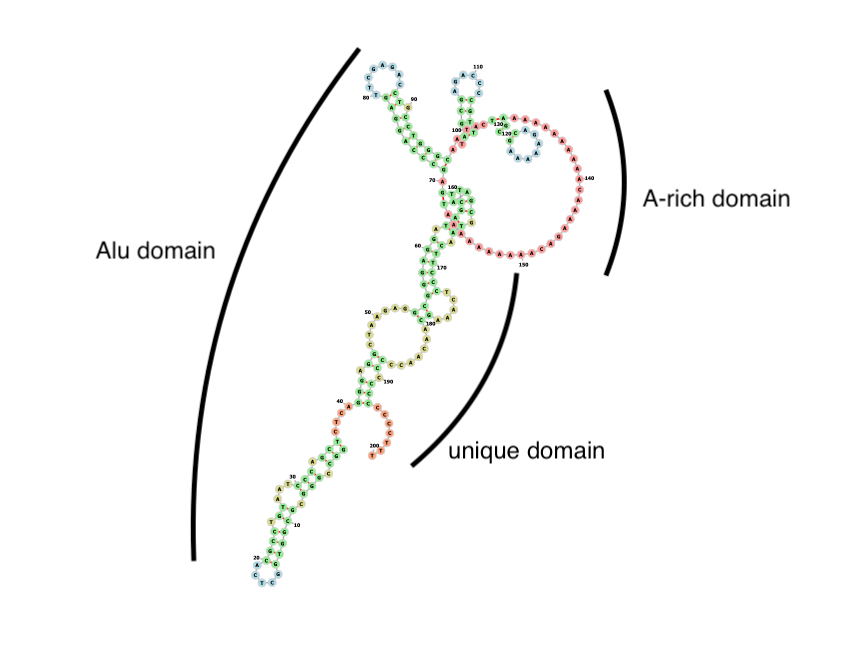
\includegraphics[width=0.4\textwidth]{figs/rna-6.png}
  \caption{BC200 RNA Secondary Structure}
  \label{fig:bc200-structure}
\end{figure}

By comparing the Alu domain of BC200 and its homologs (see Appendix \ref{app:A}), we concluded that the Alu domain between human BC200 and its selected homologs are nearly identical. 
From this conclusion, we can infer that the functions of each of the homologs may be the same as those of BC200. 
Fig. \ref{fig:gorilla-structure}, \ref{fig:pan-structure}, and \ref{fig:pongo-structure} show the RNA secondary structure of the three most closely related BC200 homologs from great apes (\emph{Hominidae}). 
Additionally, we have chosen to depict the RNA secondary structure of the \emph{Hylobates lar} BC200 homolog in Fig. \ref{fig:hylobates-structure}. 
While \emph{Hylobates lar} is not a great ape, it is still part of the \emph{Hominoidea} superfamily, and Phylogenetic analysis revealed that it was closely related to BC200.

\begin{figure*}[!h]
  \centering
  \begin{subfigure}[b]{0.4\textwidth}
    \centering
    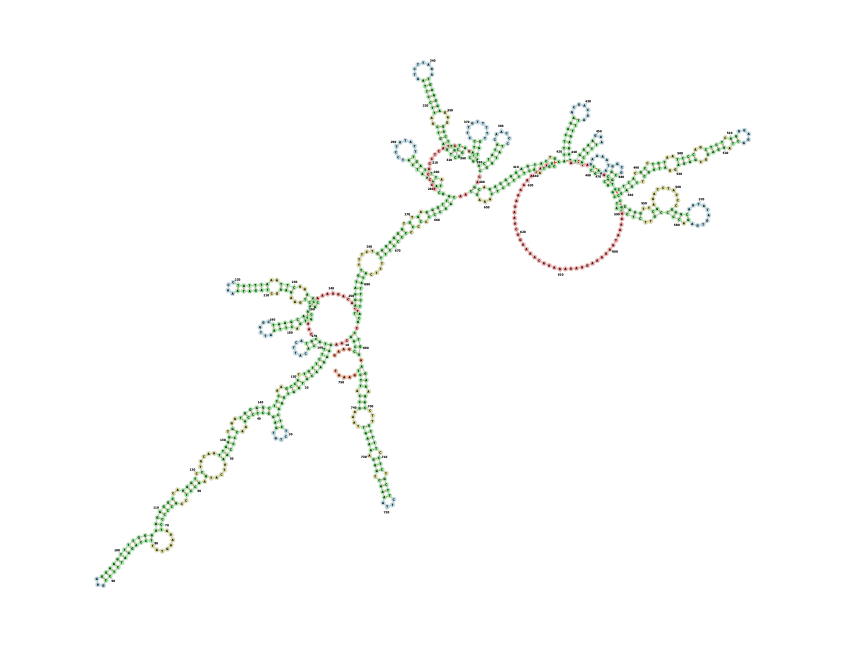
\includegraphics[width=\textwidth]{figs/rnagorilla.png}
    \caption{BC200 RNA Secondary Structure of \emph{Gorilla gorilla}}
    \label{fig:gorilla-structure}
  \end{subfigure}
  \hfill
  \begin{subfigure}[b]{0.4\textwidth}  
    \centering
    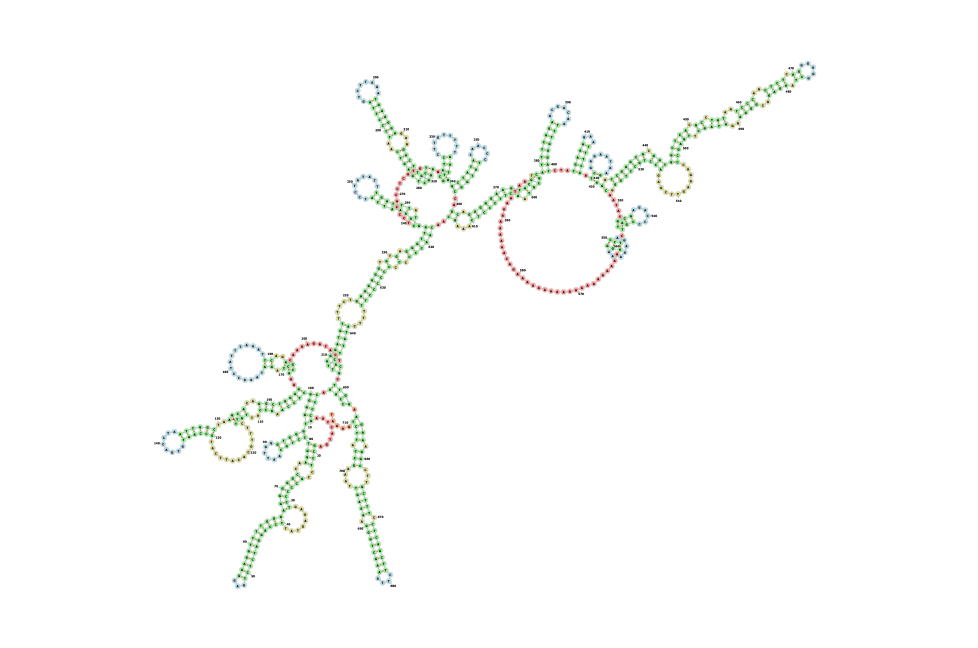
\includegraphics[width=\textwidth]{figs/rnapan.png}
    \caption{BC200 RNA Secondary Structure of \emph{Pan paniscus}}
    \label{fig:pan-structure}
  \end{subfigure}
  \vskip\baselineskip
  \begin{subfigure}[b]{0.4\textwidth}   
    \centering
    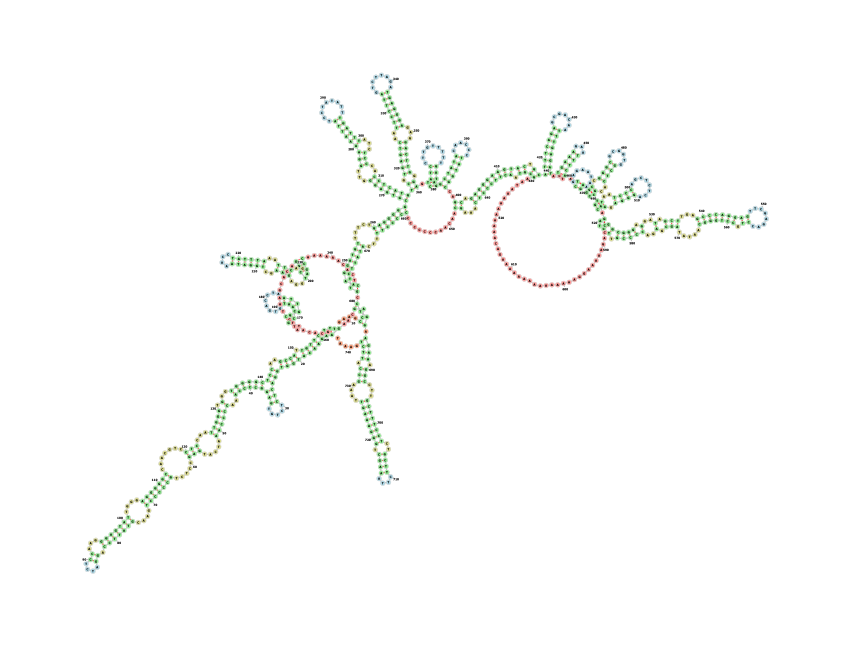
\includegraphics[width=\textwidth]{figs/rnapongo.png}
    \caption{BC200 RNA Secondary Structure of \emph{Pongo pygmaeus}}
    \label{fig:pongo-structure}
  \end{subfigure}
  \hfill
  \begin{subfigure}[b]{0.5\textwidth}   
    \centering
    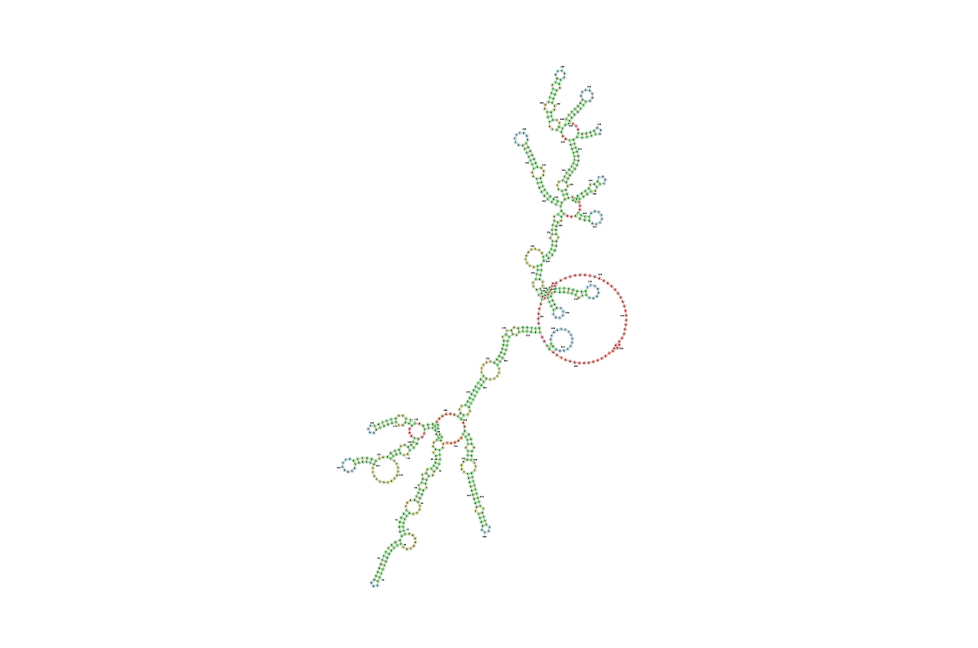
\includegraphics[width=\textwidth]{figs/rnahylobates.png}
    \caption{BC200 RNA Secondary Structure of \emph{Hylobates lar}}
    \label{fig:hylobates-structure}
  \end{subfigure}
  \caption{RNA Secondary Structures of \emph{Hominoidea} BC200 Homologs, generated by FORNA \cite{kerpedjiev2015forna} using default parameters}
  \label{fig:rna-sec-structure}
\end{figure*}

\subsection{Finding Conserved Parts of BC200}

Using multiple sequence alignment we aligned BC200 with its four mostly related homologs to find conserved parts of BC200. 
The result of the multiple sequence alignment can be found in Appendix \ref{app:B}

From the multiple sequence alignment, we can conclude that a majority (88\%) of the BC200 homolog sequences are conserved. 
Sequence conservation in non-coding RNAs is generally poor compared to protein-coding sequences, and base pairs that contribute to structure or function are often conserved instead \cite{johnsson2014evolutionary}. 
The result shows that there should be a high similarity between the function of BC200 in \emph{Homo sapiens} and closely related species. 
So, the following result does not support or refuse our hypothesis, the homologs that we found didn't have the same secondary structure, which import scoffolding function to RNA. But they had the same Alu elements, so we cannot state that whether their function is different in differenct species or not. 

\section{Discussion}\label{sec:discussion}

In this study we first began by gathering known homologs of \emph{Homo sapiens} BC200 via NCBI Blast \cite{blastTool,madden2012blast}. 
Using these homologs, we built the phylogenetic tree in order to determine which homologs were the most evolutionarily related. 
Once we had determined that the BC200 homologs from \emph{Pan paniscus}, \emph{Pongo pygmaeus}, \emph{Hylobates lar}, and \emph{Gorilla gorilla} were the most closely related to \emph{Homo sapiens} BC200, we used FORNA to determine their secondary structure \cite{lorenz2011viennarna}. 
We found that the secondary structures of \emph{Homo sapiens} BC200, shown in Fig. \ref{fig:bc200-structure}, differs from that of of \emph{Gorilla gorilla}, \emph{Pan paniscus}, and \emph{Pongo pygmaeus} BC200, shown in Fig. \ref{fig:gorilla-structure}, \ref{fig:pan-structure}, \ref{fig:pongo-structure}.
However, by comparing the Alu domains present in \emph{Homo sapiens} BC200 with the Alu domains of \emph{Gorilla gorilla}, \emph{Pan paniscus}, and \emph{Pongo pygmaeus} BC200 we can say that their gene regulation functions may be similar. 

Here we showed that several \emph{Hominoidea} homologs of BC200 share evolutionary ancestors as shown in Fig. \ref{fig:phylo-tree}. 
Additionally, we have shown that the four most closely related \emph{Hominoidea} homologs of \emph{Homo sapiens} BC200 have differing RNA secondary structures.
Although many papers suggest that beta-amyloid may cause AD, there is biological evidence that contradicts this hypothesis \cite{selkoe2016amyloid}.
As mentioned above, overexpression of BC200 will increase expression of BACE1, which in turn generates beta-amyloid. 
Despite the high similarity between BC200 lncRNA in \emph{Homo sapiens} and in \emph{Pan paniscus} and \emph{Pongo pygmaeus}, this does not definitively answer the question of whether or not AD is a uniquely human disease.
This indicates that further research in this area is needed to draw a definitive conclusion. 
Alzheimer’s disease is extremely complex and this work is only aimed determining one facet of how AD may proceed in \emph{Hominoidea} other than \emph{Homo sapiens}. 
In a recent review paper, Drummond \emph{et al.} discuss the many models of AD pathology including transgenic mice/rats, invertebrate animals, and \emph{in vitro} human cell culture models \cite{drummond2017alzheimer}. 
After reviewing the many models of AD pathology, they conclude that AD is a uniquely human disease \cite{drummond2017alzheimer}. 
Although, the conclusion of Drummond \emph{et al.} is not supported by our observations, it does not necessarily contradict it. 
Our results show that further research involving laboratory methods are necessary to understand the role of BC200 in other \emph{Hominoidea}.

\subsection{Limitations}

Our analysis began by selecting similar sequences via NCBI Blast. 
As the sequences we chose were selected based on being known BC200 homologs, we may have missed sequences which are potential homologs. 
An example is the exclusion of the bacterial artificial chromosome sequences for \emph{Pan troglodytes}. 
If we had included these sequences and were able to isolate the section of the chromosome which encodes for BC200 our Phylogenetic tree would have contained an extra data point.
After performing phylogenetic analysis, we built the RNA secondary structure of BC200 and its homologs. 
These structures have not been experimentally confirmed and are based on the minimum free energy. 
Consequently, the structures are approximations are should be thought of as such.

\section{Conclusion}\label{sec:conclusion}

In this paper, we set out to determine if there was bioinformatic evidence that supports the hypothesis that AD is uniquely human. 
In order to determine if such evidence exists we first performed phylogenetic analysis to determine candidate species for RNA secondary structure analysis. 
Once we had determined the RNA secondary structure for the four most closely related \emph{Hominoidea} homologs of BC200, we compared their secondary structures to the secondary structure of \emph{Homo sapiens} BC200. 
We determined that the Alu domain of \emph{Homo sapiens}, \emph{Pan paniscus}, and \emph{Pongo pygmaeus}, \emph{Gorilla gorilla} and \emph{Hylobates lar} BC200 are structurally similar. 
Further analysis determined that 88\% of \emph{Homo sapiens} BC200 sequence is conserved during evolution, as shown in Appendix \ref{app:B}. 
While much of the \emph{Homo sapiens} BC200 sequence is conserved, the BC200 homologs were much longer than that of \emph{Homo sapiens} BC200.
The result of a different RNA secondary structure may suggest that BC200 has a different regulatory function each host organism.
Other results, including having the same Alu domains, the connection of each homolog through the phylogenetic tree, and the existence of a large portion of conserved nucleotides in BC200, suggests that their function may be similar. 
In conclusion, our analysis of BC200 homologs in \emph{Hominoidea} suggest that they may have conserved function in the body, but that more research on the topic is required to determine if AD is uniquely human.

\bibliographystyle{IEEEtran}
\bibliography{refs.bib}

\vspace{4cm}

\onecolumn
\appendices


\includepdf[pages=-, height=0.8\paperheight, pagecommand=\section{Dfam Analysis of Alu Domains}\label{app:A}\subsection{\emph{Homo sapiens}}]{figs/human-bc200-alu-domain.pdf}

\includepdf[pages=-, height=0.8\paperheight, pagecommand=\subsection{\emph{Gorilla gorilla}}]{figs/gorilla-bc200-alu-domain.pdf}

\includepdf[pages=-, height=0.8\paperheight, pagecommand=\subsection{\emph{Pan paniscus}}]{figs/pan-bc200-alu-domain.pdf}

\includepdf[pages=-, height=0.8\paperheight, pagecommand=\subsection{\emph{Pongo pygmaeus}}]{figs/pongo-bc200-alu-domain.pdf}

\section{ClustalW Multiple Sequence Alignment of BC200 and \emph{Hominoidea} Homologs}
\label{app:B}

\begin{figure}[ht]
  \centering
  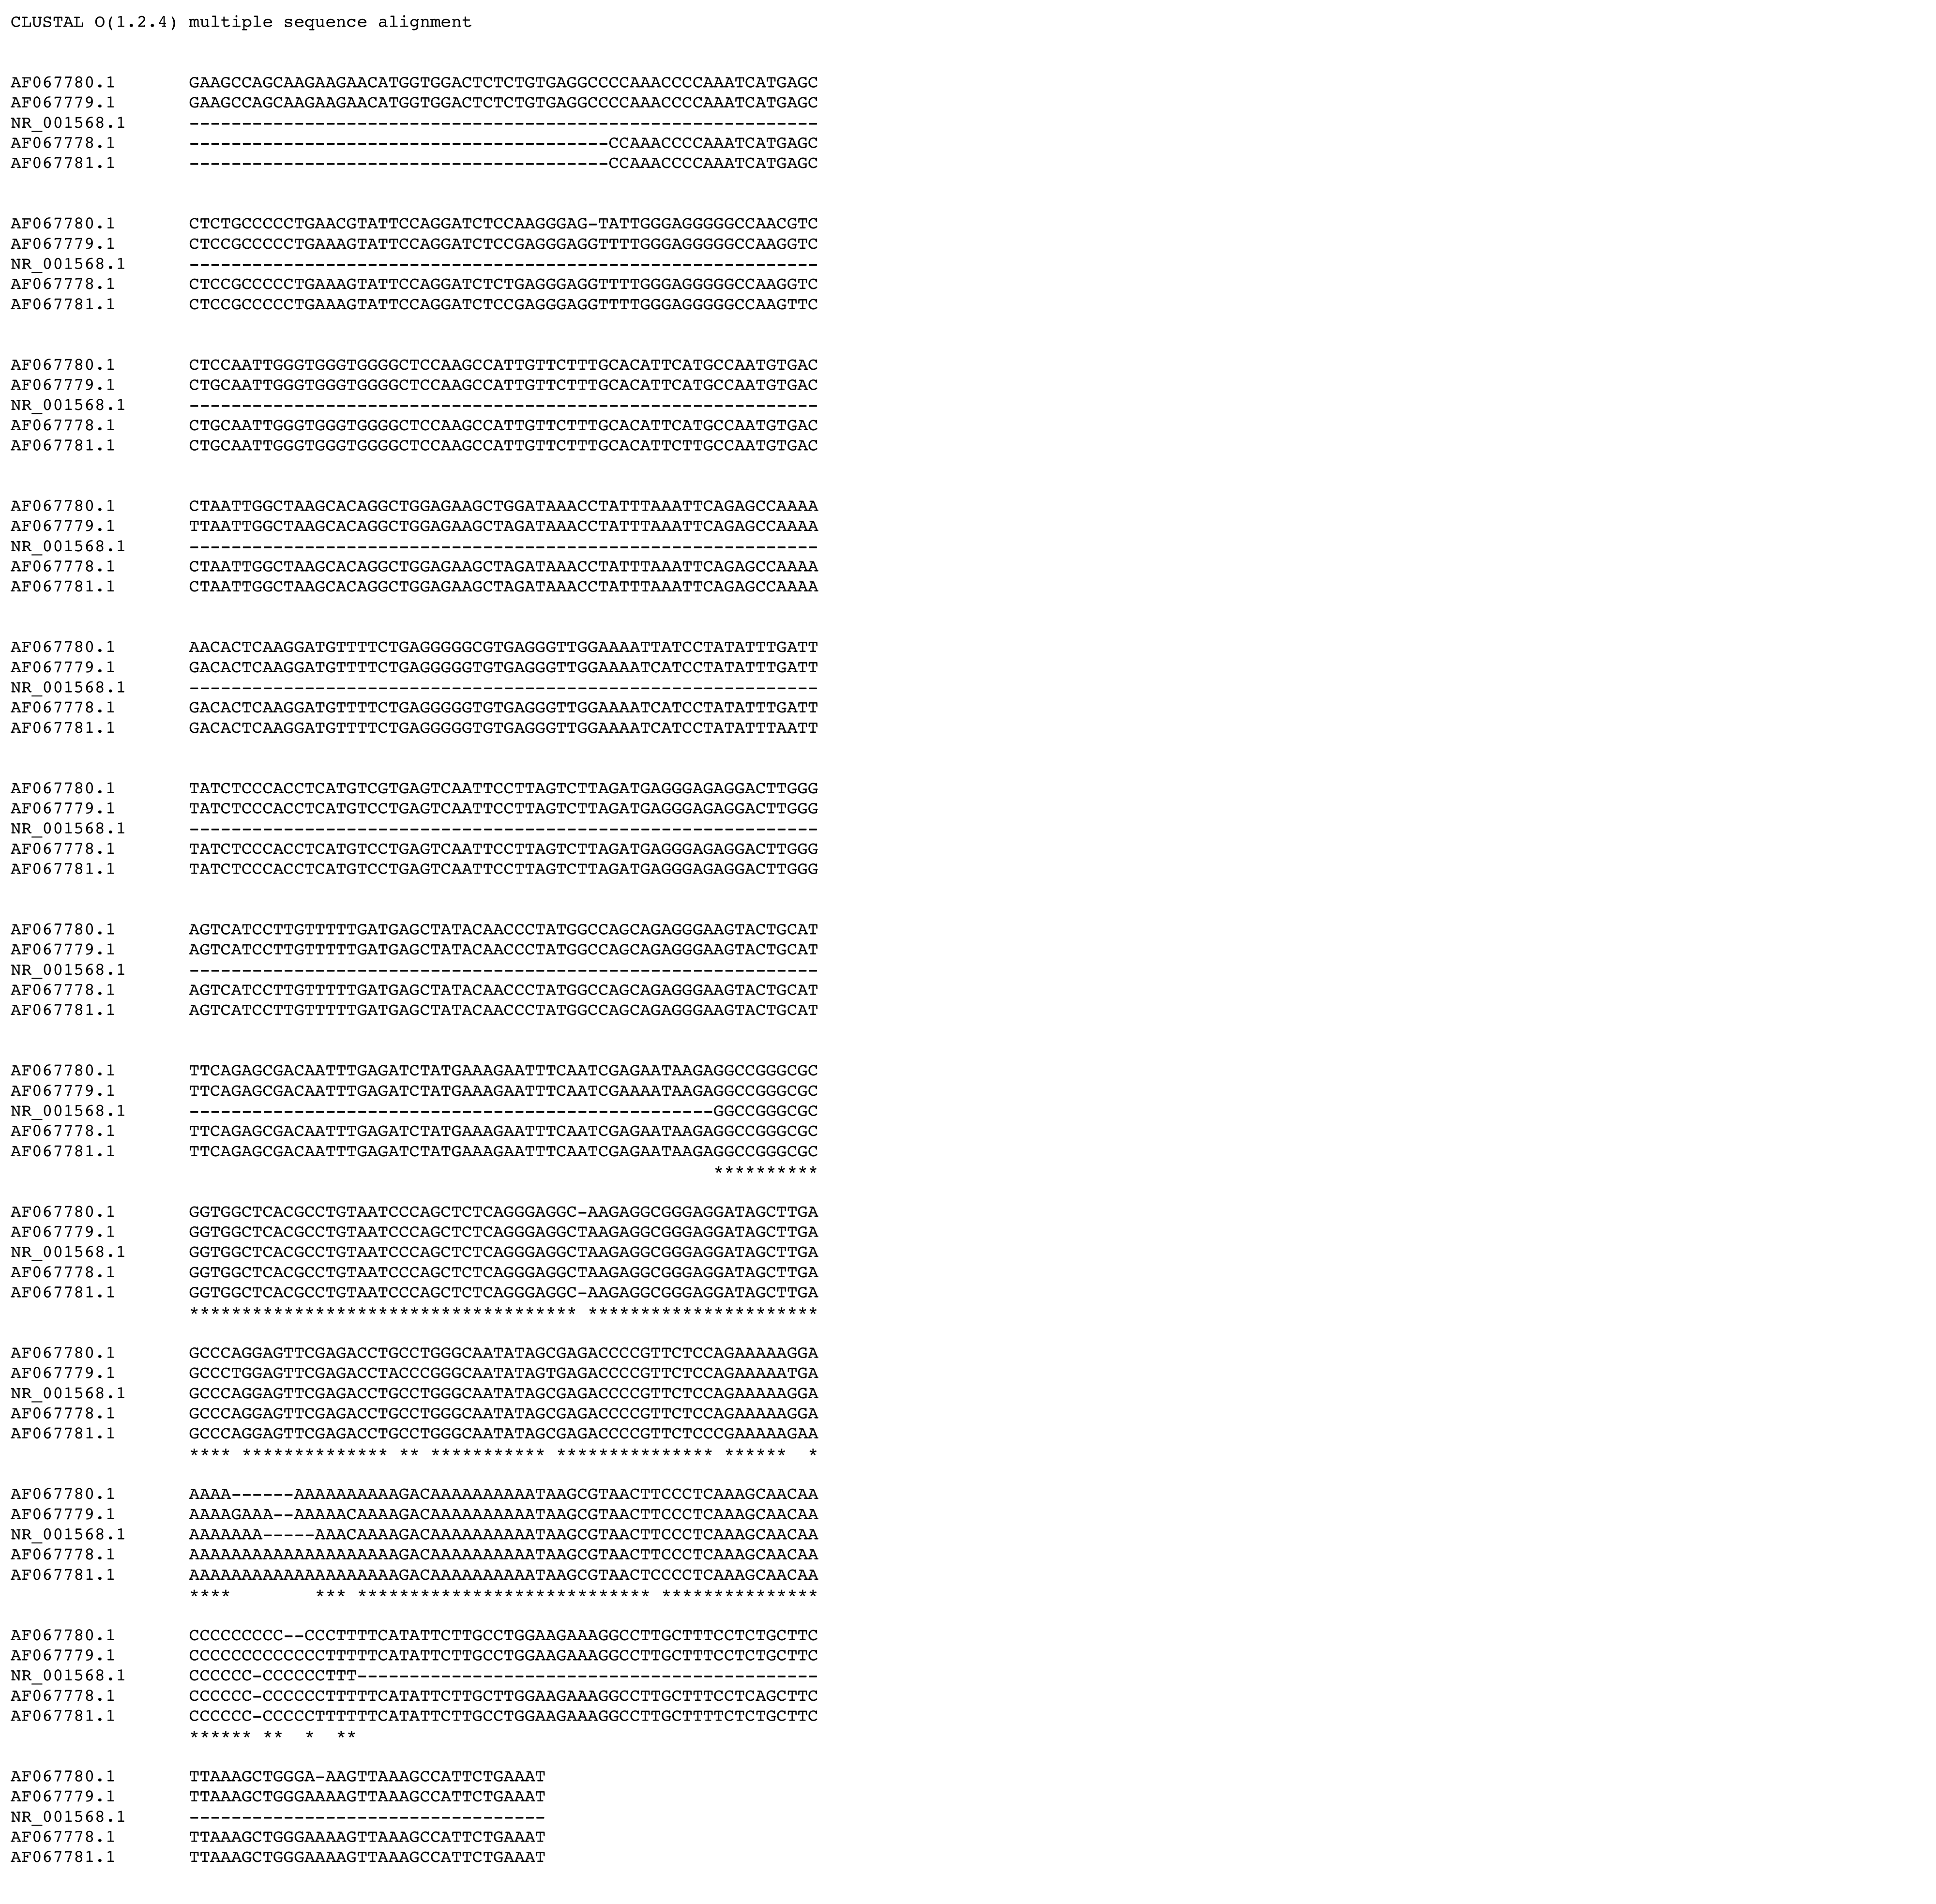
\includegraphics[height=0.825\textheight, width=\textwidth, keepaspectratio]{figs/alignment.png}
\end{figure}

\end{document}
